\documentclass[12pt,a4paper]{article}
\usepackage{txfonts}
\usepackage{url}
\usepackage[colorlinks, citecolor=blue, urlcolor=blue]{hyperref}
\usepackage[utf8]{inputenc}
\usepackage[spanish]{babel}
\usepackage{amsmath}
\usepackage{amsfonts}
\usepackage{amssymb}
\usepackage{makeidx}
\usepackage{graphicx}
\usepackage{lmodern}
\usepackage{kpfonts}
\usepackage{fourier}
\usepackage[left=2cm,right=2cm,top=2cm,bottom=2cm]{geometry}
\author{Rodriguez Lopez Francisco Javier}
\begin{document}

\begin{center}
\LARGE \textbf{Universidad Politecnica de la Zona Metropoilitana de Guadalajara\\}



\includegraphics[scale=1]{Upzmg6.png} 

\large \textbf{Diseño de un PWM con Amp-op y Transistores}\\
\vspace{2cm}
\large \textbf{Nombre: Rodriguez Lopez Francisco Javier.\\
\vspace{0.5cm} Matricula: 18311804.\\
\vspace{0.5cm} Carrera: Ingenieria en Mecatronica.\\
\vspace{0.5cm} Materia: Sistemas Electronicos de Interfaz.\\
\vspace{0.5cm} Curso: septiembre-diciembre del 2019.\\
\vspace{0.5cm} Docente: Moran Garabito Carlos Enrique.}


\vspace{6cm}
\small \textbf{22 de Octubre del 2019}
\end{center}

\section{Diseño de un PWM apartir de amplificador y transistor:}

La modulacion de pulso llamada por sus siglas PWM, es objeto de gran ayuda en convertidores de voltaje, ya que como sabemos un amplificador operacional, es adaptado para que las ondas generadas  partir de la entrada sean mayores ya cuando estas van de salida, siendo esta la modulacion de pulso electrico que pueda recibir a partir de captaciones de movimkento de corriente que esta pueda fluir y pueda ser de mayor impulso y de otra manera el pulso generado a partir de la entrada.\\

Ahora por otra parte se encuentra los transistores, en este caso,al ser llamados transiciones de corriente dependiendo en este caso la corriente con la que se activa dicho transistor, ya sea este PNP o NPN, sera la conmutaacion que este tenga con el circuito en si, para la solucion de ese problema que conmunmente se regula, que es el de la insuficiencia en la parte de corriente, llevado a cabo por este dispositivo.\\

Lo que se estara viendo en esta Redaccion, es ver el esquematico empleaod por el servidor escritor de este texto, para la buena solucion en explicacion de lo que consta la tarea, y como estos componentes juntos, nos pueden dar un PWM, de buen uso, y de buena amplificacion regulando, las entradas y salidas.\\

\begin{center}
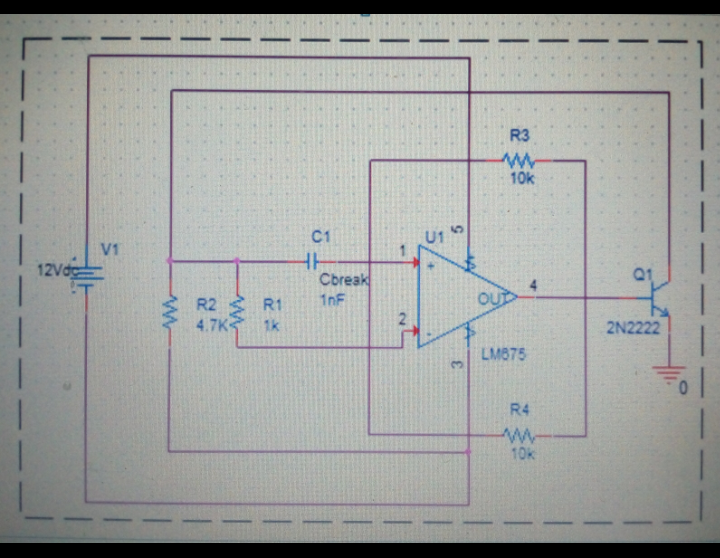
\includegraphics[width=10cm]{diagrama.png} 
\end{center}

En el diagrama que se muestra en la imagen superior, se ve lo que en constancia nos pide la tarea, que es ver la acoplacion de los amplificadores operacionales, en conjunto con los transistores, para asi poder crear una modulacion de pulso respecto a la constancia de voltaje que se este manejandon en este caso es de 12 voltios.\\

Se le llama modulacion de pulso, por que sus fases entre las ondas, se empiezan a disminuir y a agrandar respectivamente despues de un tempo de la amplificacion dda, la condensacion que se encuentra en el inicio, como se muestra de igual forma, hay un puente de resistencias, las cuales, nos dejan apreciar, como esta generacion de corriente es mas controlada, repsecto a la emision de entrada, que esta dada, conectada, directamente a la resistencia que esta conectada al ccondensador, para llevar a la pata del emsior del transistor, esto para que el flujo de la onda se expanda y generar lo que en pirncipio se situa esta practica, que es ver la amplificacion dada por el V1, y el VOUT, cada uno repsectivamente trabajando en el ya mencionado emisor.\\

Por otra parte se ve, la parte del conector, este casi en todos los casos se va a tierra y esta no es la excepcion, ya que en esta parte es cuando la onda generada, a partir de la descarga del condensador, sutado en la resitencia uno, hace que genere una onda mas peqyeña, en este caso, ya sea cuadratica, o senoidal. En otod sistema, siempre hay este tipo de situaciones, ya que el amplificador, hace su trabajo, que es situar cada una de las corrientes, ya sea en este caso, en el emsior o conector del transistor, y cuando es que este empieza a dar ese tipo de señales recabadas en terminos mas sencillos los de la generacion de ondas corta/amplia.\\

Mas en concreto se utiliza el transistor, para regular la potencia disipada en el circuito, en dado caso de que las cargas sean pesadas, y de un rango mayor, como se puede mostrar en el desfase de ondas generadas a partir del voltaje que este reciba.\\

En dado caso, de que se puedan mostrar fallas, o concretas situaciones de riesgo para los componentes, se puede colocar de antemano, un triac, el cual se coloca en la base del transistor, esto para que su voltaje dada la salida de voltaje(VOUT), no estropie las señales y la generacion de un buen desfase, y en cambio de ello nos encare con armonicos de mucho ruido, y de generacion de corriente mayor, que pueda estropear nuestros componentes, dejando asi, un margen mayor de confianza, para este diagrama se puede utlizar un condensador de 1uF, a 50v, esto para que la atenuacion de ondas, sea evidente, y no interfiera mucho en la entrada de voltaje, conectando el positivo del amplificador al positivo de la fuente, y el negativo de la guente con el negativo del amplificador.\\

\begin{center}
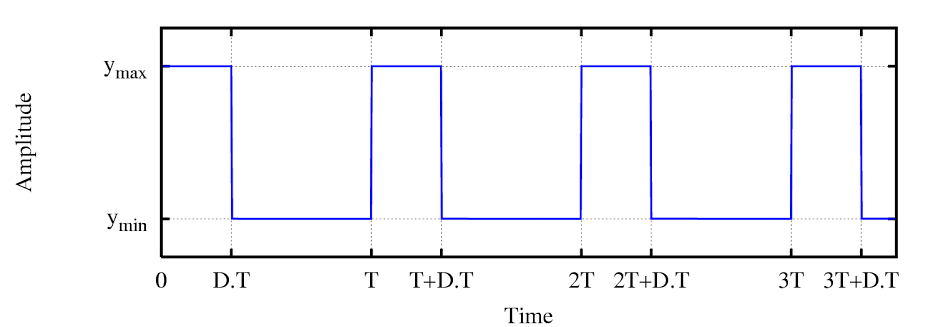
\includegraphics[width=12cm]{onda.png} 
\end{center}

En la imagen posterior, muestra las ondas, en ejemplo que nos puede lanzar las fases de la amplificacion con el transistor, dandonos asi una modulacion de ondas en pulso, respecto al tiempo ya sea en este caso, la variable del condensador, y del transistor, o en otro caso, la misma fuente de alimentacion, que nos deja ver con pre-angulo, la generacion de las ondas, en este caso cuadraticas, por el mismo modulo de pulso generado a partir de las conexiones y sus componentes enlazados.

Se debe de aparentar un movimiento en la fase de las ondas, como si estas abrieran y cerraran, por la descarga y carga que tiene comunmente el condensador, regulando a partir de las resistencias una buena corriente y armonicos lanzados, y de otra forma, la generacion de la amplificacion con comunicacion con el transistor, y esto a su vez por el emisor y el conector.\\

Se pueden establecer, mas variables que ayuden a la mejora de la ejecucion de este diagrama, o circuito, pero por el momento solo se busca la explicacion del modulo de pulso que se recibe a partir de la generacion de carga que la fuente de aliemntacion propaga en el sistema.
\newpage

\textbf{\LARGE Referencias Bibliograficas:}\\

\url{http://digital.ni.com/public.nsf/allkb/AA1BDEA4AA224E3E86257CE400707527}

\end{document}